\documentclass{ximera}

\begin{document}
\begin{problem}
  The number $x$ is shown below on a number line.
  \begin{image}
    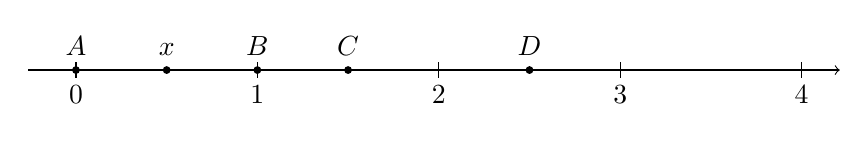
\begin{tikzpicture}[x=0.19\textwidth]
      \draw[-{>[scale=1.75]}] (-0.05\textwidth,0) -- (0.8\textwidth,0);
      \foreach \x in {0,...,4} {%
        \draw (\x,-.1) -- (\x,.1);
        \node[anchor=north,yshift=-2pt] at (\x,0) {$\x$};
      }
      \draw (0.5,0) node [circle,fill,inner sep=1pt,label=above:$x$](e){};
      \draw (0,0) node [circle,fill,inner sep=1pt,label=above:$A$](e){};
      \draw (1,0) node [circle,fill,inner sep=1pt,label=above:$B$](e){};
      \draw (1.5,0) node [circle,fill,inner sep=1pt,label=above:$C$](e){};
      \draw (2.5,0) node [circle,fill,inner sep=1pt,label=above:$D$](e){};
    \end{tikzpicture}
  \end{image}
  Which number is closer to $\sqrt{x}$?
  \begin{multipleChoice}
    \choice{$A$}
    \choice[correct]{$B$}
    \choice{$C$}
    \choice{$D$}
  \end{multipleChoice}
\end{problem}
\end{document}
